\documentclass[aspectratio=169, table]{beamer}
\usepackage[utf8]{inputenc}
\usepackage{listings} 
\usepackage[strings]{underscore}
\usepackage{caption}

\renewcommand{\lstlistingname}{} 

\makeatletter
\def\input@path{{../../themes/Pradita}}
\makeatother

\usetheme{Pradita}

\subtitle{IF120203-Programming Fundamentals}

\title{Chatper-02:\\\LARGE{Variabel, Konstanta, Tipe Data,\\ dan Konversi Tipe Data}}
\date[Serial]{\scriptsize {PRU/SPMI/FR-BM-18/0222}}
\author[Pradita]{\small{\textbf{Alfa Yohannis}}}


% Define Python language style for listings
\lstdefinestyle{PythonStyle}{
language=Python,
basicstyle=\ttfamily\footnotesize,
keywordstyle=\color{blue},
commentstyle=\color{gray},
stringstyle=\color{red},
breaklines=true,
showstringspaces=false,
tabsize=2,
captionpos=b,
numbers=left,
numberstyle=\tiny\color{gray},
comment=[l]{//},
morecomment=[s]{/*}{*/},
commentstyle=\color{gray}\ttfamily,
string=[s]{'}{'},
morestring=[s]{"}{"},
}

\begin{document}

\frame{\titlepage}

% Add table of contents slide
\begin{frame}[fragile]{Contents}
\vspace{15pt}
\begin{columns}[t]
\begin{column}{.5\textwidth}
\tableofcontents[sections={1-3}]
\end{column}
\begin{column}{.5\textwidth}
\tableofcontents[sections={4}]
\end{column}
\end{columns}
\end{frame}

\section{Variabel}
\begin{frame}{Apa Itu Variabel?}
Variabel merupakan tempat penyimpanan sementara yang digunakan untuk menampung data selama program berjalan, sehingga data tersebut dapat digunakan kembali. Berbeda dengan bahasa pemrograman \textit{static type} seperti C, C++, dan Java yang harus secara eksplisit menulis tipe data untuk variabel. Di Python, variabel memiliki tipe data yang dinamis (\textit{dynamic type}) dan dapat berubah sesuai dengan kebutuhan program.
\end{frame}

\begin{frame}{Analogi Variabel}
\begin{figure}[H]
	\centering
	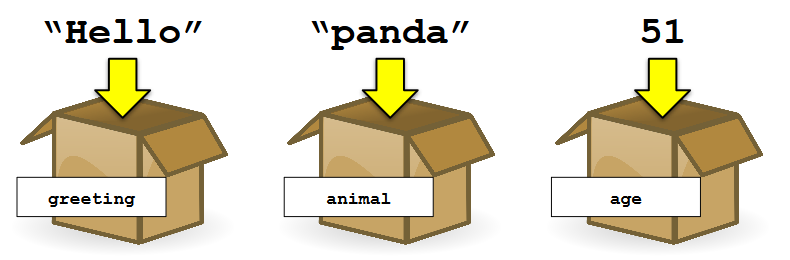
\includegraphics[width=0.7\textwidth]{assets/images/variable_analogy.png}
	\caption*{\textbf{Gambar 1:} Analogi Variabel Sebagai Sebuah Box}
	\smallskip
    {\tiny Sumber: \url{https://aljebraschool.hashnode.dev/python-for-machine-learning}}
\end{figure}
\end{frame}

\begin{frame}{Struktur Variabel}
\begin{figure}[H]
	\centering
	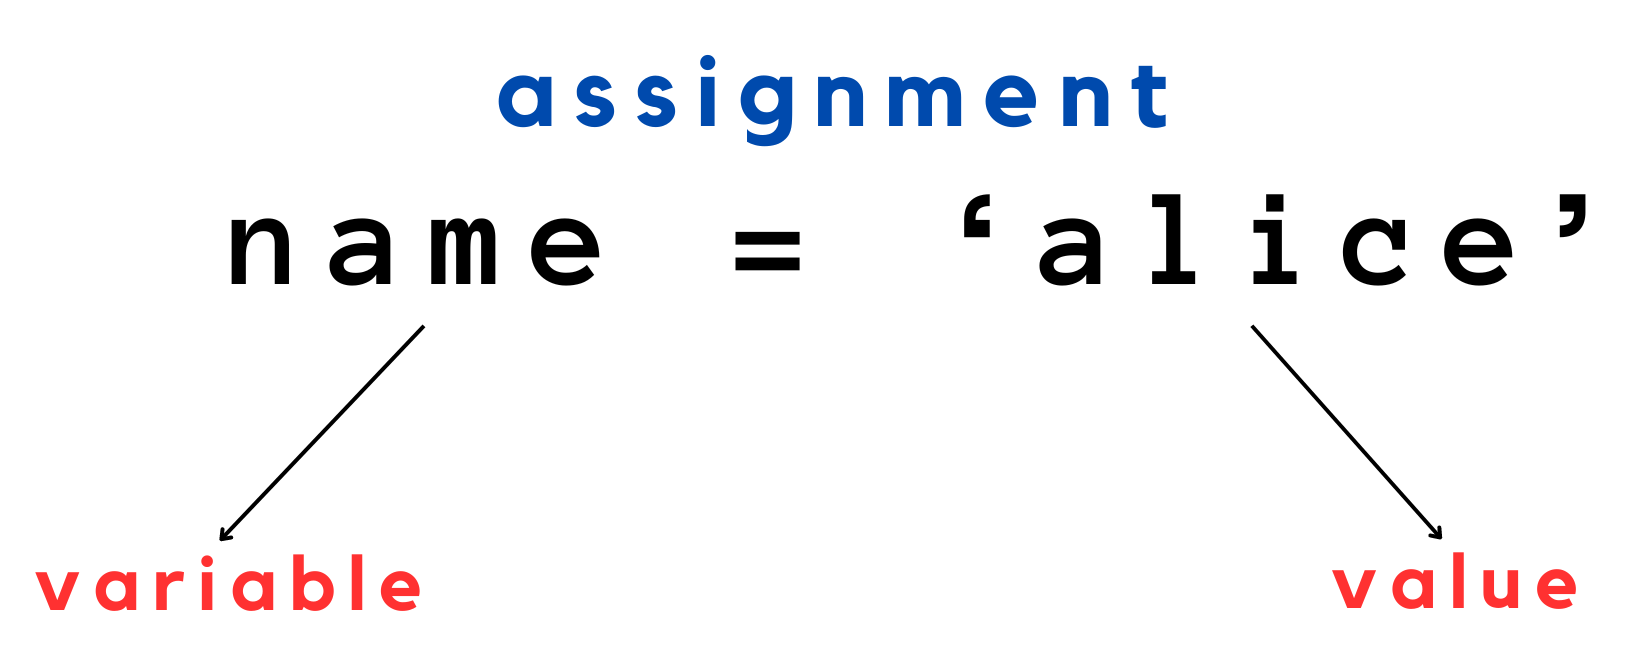
\includegraphics[width=0.7\textwidth]{../../../shared_assets/images/python_variable_structure.png}
	\caption{}
	\caption*{\textbf{Gambar 2:} Struktur Variabel di Python}
	\smallskip
    {\tiny Sumber: \url{https://www.ankitweblogic.com/c/compiler-and-interpreter.php}}
\end{figure}
\end{frame}

\begin{frame}{Aturan Penamaan Variabel}
\begin{itemize}
\item Nama variabel harus dimulai dengan huruf atau underscore (\_).
\item Nama variabel tidak boleh dimulai dengan angka.
\item Nama variabel tidak boleh mengandung spasi.
\item Nama variabel tidak boleh mengandung simbol.
\item Nama variabel tidak boleh mengandung kata kunci (\textit{keyword}) yang sudah terdefinisi dalam Python, seperti \texttt{def}, \texttt{for}, \texttt{if}, \texttt{return}, dan sebagainya.
\end{itemize}
\end{frame}

\begin{frame}[fragile]{Latihan Membuat Variabel}
\begin{lstlisting}[style=PythonStyle, caption={Kode Python: variable.py}]
nama = "Stefani Laurensia"
usia = 21
berat_badan = 50.2

print(nama)
print(usia)
print(berat_badan)
\end{lstlisting}
\end{frame}

\begin{frame}[fragile]{Contoh Kesalahan Penamaan Variabel}
\begin{lstlisting}[style=PythonStyle, caption={Kode Python: variable.py}]
1angka = 200 # Nama variabel tidak boleh dimulai dengan angka
nama lengkap = "Budi" # Nama variabel tidak boleh mengandung spasi
gaji$ = 1000000 # Nama variabel tidak boleh mengandung simbol
class = "Informatika" # class merupakan reserved keyword di Python
\end{lstlisting}
\end{frame}

\section{Konstanta}
\begin{frame}{Apa Itu Konstanta?}
Konstanta adalah variabel yang seharusnya nilainya tidak berubah selama program berjalan. Contohnya nilai \textbf{\textit{pi}} (3.14) atau gravitasi (9.81). Di Python, kita bisa menandai variabel sebagai Final dari modul \texttt{typing} untuk memberi tanda bahwa variabel tersebut dimaksudkan sebagai konstanta.
\end{frame}

\begin{frame}{Hal-hal yang Perlu Diperhatikan}
\begin{itemize}
\item Python tidak memaksa variabel \texttt{Final} agar tidak bisa diubah.
\item Penandaan \texttt{Final} hanya \textbf{memberi peringatan pada type checker}, bukan mencegah perubahan di runtime.
\end{itemize}
\end{frame} 

\begin{frame}{Aturan Penamaan Konstanta}
\begin{itemize}
\item Untuk menandakan bahwa sebuah variabel adalah konstanta, kita bisa menggunakan huruf besar untuk membedakan dengan variabel biasa.
\item Hal ini mengikuti aturan penamaan variabel yang dibuat oleh Python (\href{https://peps.python.org/pep-0008/}{PEP 8 - Style Guide for Python Code}).
\end{itemize}
\end{frame}

\begin{frame}[fragile]{Latihan Membuat Konstanta}
\begin{lstlisting}[style=PythonStyle, caption={Kode Python: constant.py}]
from typing import Final

PI: Final = 3.14
GRAVITASI: Final = 9.81

print(PI)
print(GRAVITASI)

GRAVITASI = 10 # Nilai masih tetap bisa berubah, tapi tidak disarankan
print(GRAVITASI)
\end{lstlisting}
\end{frame}

\section{Tipe Data}
\begin{frame}{Apa Itu Tipe Data?}
Tipe data merupakan jenis data yang bisa disimpan di program Python. Tipe data di Python memiliki banyak jenis, seperti \texttt{int}, \texttt{float}, \texttt{str}, \texttt{bool}, \texttt{list}, \texttt{tuple}, \texttt{dict}, dan \texttt{set}. Namun pada \textit{chapter} kali ini, kita akan fokus pada tipe data dasar, antara lain \texttt{int}, \texttt{float}, \texttt{str}, dan \texttt{bool}.
\end{frame}

\begin{frame}{Tipe Data di Python}
\begin{figure}[H]
	\centering
	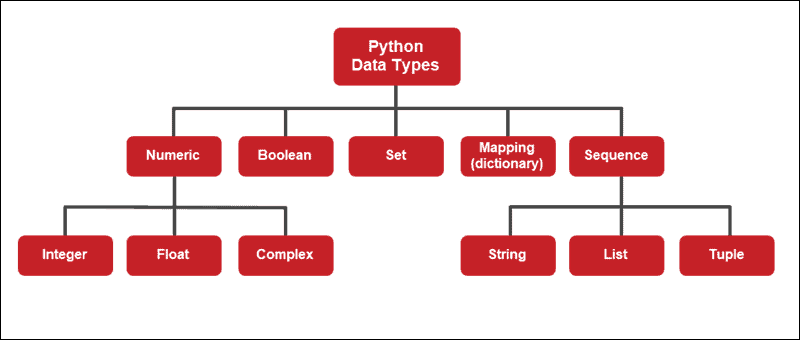
\includegraphics[width=0.7\textwidth]{assets/images/python_data_types.png}
	\caption*{\textbf{Gambar 3:} Macam-macam tipe data di Python}
	\smallskip
    {\tiny Sumber: \url{https://aljebraschool.hashnode.dev/python-for-machine-learning}}
\end{figure}
\end{frame}

\begin{frame}[fragile]{Tipe Data Berdasarkan Kelompoknya (1)}
\begin{itemize}
\item \textbf{Numeric} (Angka)
\begin{enumerate}
\item \textbf{Integer} (bilangan bulat)
\begin{lstlisting}[style=PythonStyle]
usia = 18
jumlah_mahasiswa = 64
nomor_rumah = 88

suhu = -5
\end{lstlisting}
\item \textbf{Float} (bilangan desimal)
\begin{lstlisting}[style=PythonStyle]
koordinat_x = 5.5
koordinat_y = 7.8

saldo = 10.500.075
\end{lstlisting}
\end{enumerate}

\end{itemize}
\end{frame}

\begin{frame}[fragile]{Tipe Data Berdasarkan Kelompoknya (2)}
\begin{itemize}
\item \textbf{String} (Kata / Kalimat)
\begin{lstlisting}[style=PythonStyle]
nama = "John"
quote = 'Programmer: A machine that turns coffee into code'
pesan_email = """
Kepada Yth. John Doe,

Terima kasih atas pesanan anda.
"""
\end{lstlisting}

\end{itemize}
\end{frame}

\begin{frame}[fragile]{Tipe Data Berdasarkan Kelompoknya (3)}
\begin{itemize}
\item \textbf{Boolean} (Benar atau Salah)
\begin{lstlisting}[style=PythonStyle]
is_married = False
is_single = True
\end{lstlisting}

\end{itemize}
\end{frame}

\section{Konversi Tipe Data (\textit{Type Casting})}

\begin{frame}{Apa Itu Konversi Tipe Data?}
Kadang kita perlu mengubah tipe data dari satu jenis ke jenis lain agar Python bisa memprosesnya dengan benar.
Misal, input dari pengguna melalui fungsi \texttt{input()} selalu mengembalikan tipe data string (str), tapi kita ingin melakukan perhitungan angka, maka kita harus mengubahnya menjadi int atau float.
\end{frame}

\begin{frame}{Fungsi Untuk Konversi Tipe Data di Python}
\begin{figure}[H]
	\centering
	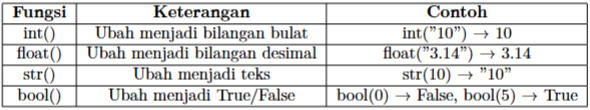
\includegraphics[width=0.7\textwidth]{assets/images/type_casting_function.png}
	\caption*{\textbf{Gambar 4:} Tabel Fungsi Untuk Konversi Tipe Data di Python}
\end{figure}
\end{frame}

\begin{frame}[fragile]{Latihan Konversi Tipe Data (1)}
\begin{lstlisting}[style=PythonStyle, caption={Kode Python: string_to_int.py}]
usia = input("Masukkan usia Anda: ")
print("Tipe data sebelum konversi:", type(usia)) # Menampilkan tipe data sebelum konversi

usia = int(usia) # Konversi tipe data string menjadi integer
print("Tipe data setelah konversi:", type(usia)) # Menampilkan tipe data setelah konversi

usia_lima_tahun_kemudian = usia + 5 # Perhitungan usia 5 tahun kemudian
print("Usia 5 tahun kemudian:", usia_lima_tahun_kemudian)
\end{lstlisting}
\end{frame}

\begin{frame}[fragile]{Latihan Konversi Tipe Data (2)}
\begin{lstlisting}[style=PythonStyle, caption={Kode Python: string_to_float.py}]
angka_str = "45.67"
print("Sebelum konversi:", angka_str, type(angka_str))

angka_float = float(angka_str)
print("Setelah konversi ke float:", angka_float, type(angka_float))
\end{lstlisting}
\end{frame}

\begin{frame}[fragile]{Latihan Konversi Tipe Data (3)}
\begin{lstlisting}[style=PythonStyle, caption={Kode Python: int_to_float.py}]
angka_int = 10
print("Sebelum konversi:", angka_int, type(angka_int))

angka_float = float(angka_int)
print("Setelah konversi ke float:", angka_float, type(angka_float))
\end{lstlisting}
\end{frame}

\begin{frame}[fragile]{Latihan Konversi Tipe Data (4)}
\begin{lstlisting}[style=PythonStyle, caption={Kode Python: float_to_int.py}]
angka_float = 3.99
print("Sebelum konversi:", angka_float, type(angka_float))

angka_int = int(angka_float)
print("Setelah konversi ke integer:", angka_int, type(angka_int))
\end{lstlisting}
\end{frame}

\begin{frame}[fragile]{Kesalahan dalam Konversi Tipe Data (1)}
Meskipun Python menyediakan fungsi bawaan untuk mengubah tipe data (\texttt{int()}, \texttt{float()}, \texttt{str()}, \texttt{bool()}), \textbf{tidak semua konversi bisa dilakukan dengan sukses}. Jika nilai yang dikonversi tidak sesuai dengan tipe data tujuan, maka program akan menghasilkan \textbf{error}. Berikut adalah contoh kesalahan dalam konversi tipe data:
\end{frame}

\begin{frame}[fragile]{Kesalahan dalam Konversi Tipe Data (2)}
\begin{lstlisting}[style=PythonStyle]
# String huruf → Integer
huruf = "abc"
huruf_integer = int(huruf)  
# Output: ValueError: invalid literal for int() with base 10: 'abc'

# String bilangan desimal → Integer
angka_str = "12.34"
angka_int = int(angka_str)  
# Output: ValueError: invalid literal for int() with base 10: '12.34'
\end{lstlisting}
\end{frame}

\section{Soal Latihan}
\begin{frame}{Soal Latihan (1)}
Berikut adalah beberapa soal latihan tambahan untuk menguji pemahaman Anda mengenai konsep variabel, konstanta tipe data, dan konversi tipe data yang telah dipelajari:
\end{frame}

\begin{frame}[fragile]{Soal Latihan (2)}
\begin{itemize}
\item \textbf{Soal 1:} Buat program bernama \texttt{luas_persegi_panjang.py} yang meminta pengguna memasukan nilai panjang dan lebar persegi panjang, kemudian program harus bisa menghitung dan mencetak luas persegi panjang tersebut.
\newline \newline
\textbf{Hint:} Gunakan operator perkalian \texttt{*} untuk menghitung luas.

\item \textbf{Soal 2:} Buat program bernama \texttt{luas_lingkaran.py} yang meminta pengguna memasukan nilai jari-jari lingkaran. Program harus menampung nilai konstanta \textbf{\textit{pi}} mengikuti standar \textit{best practice} dari Python dan bisa menghitung sekaligus mencetak luas lingkaran tersebut.

\end{itemize}
\end{frame}

\begin{frame}[fragile]{Soal Latihan (3)}
\begin{itemize}
\item \textbf{Soal 3:} Buat program bernama \texttt{tebak_usia.py} yang meminta pengguna memasukkan tahun lahirnya. Program harus:
\begin{enumerate}
    \item Menyimpan tahun lahir di variabel.
    \item Mengubah input dari string menjadi integer.
    \item Menghitung umur dengan mengurangi tahun saat ini dengan tahun lahir yang dimasukan oleh pengguna.
    \item Menampilkan pesan seperti: "Kamu berusia [umur] tahun."
\end{enumerate}

\textbf{Hint:} Gunakan operator pengurangan \texttt{-} untuk menghitung usia saat ini.
\end{itemize}
\end{frame}

\section{Penutup}
\begin{frame}[fragile]{Penutup}
\begin{itemize}
    \item Variabel digunakan untuk menyimpan data yang dapat berubah nilainya, sedangkan konstanta menyimpan nilai yang tetap.
    \item Python mendukung berbagai tipe data dasar, seperti \texttt{int}, \texttt{float}, \texttt{str}, dan \texttt{bool}.
    \item Konversi tipe data memungkinkan perubahan nilai dari satu tipe data ke tipe lain, namun harus hati-hati karena bisa menyebabkan error bila tidak sesuai.
\end{itemize}
\end{frame}

\end{document}